\documentclass[a4paper]{article}

%% Language and font encodings\textbf{}
\usepackage[english]{babel}
\usepackage[utf8x]{inputenc}
\usepackage[T1]{fontenc}
\usepackage{graphicx}
%% Sets page size and margins 
\usepackage[a4paper,top=0.7cm,bottom=2cm,left=3cm,right=3cm,marginparwidth=1.75cm]{geometry}

%% Useful packages
\usepackage{amsmath}
\usepackage{graphicx}
\usepackage[colorinlistoftodos]{todonotes}
\usepackage[colorlinks=true, allcolors=blue]{hyperref}


\title{Universidad Nacional Autónoma de México\\ Facultad de Ciencias\\ \Large{Sistemas Operativos 2018-2\\Android}}
\date{7 de junio de 2018}
\author{Profesor Salvador López Mendoza\\Alumnos: Grupo 1 }
\begin{document}
\maketitle

\section{Introduction}

Esta investigación es grupal sobre el sistema operativo de celular llamado Android, para tener una idea general sobre este sistema popular.
% * <razielmcr1@ciencias.unam.mx> 2018-06-07T14:30:23.421Z:
%
% ^.
\section{Temario}

\subsection{Arquitectura}
\begin{itemize}
\item Author : Acevedo Badillo Osvaldo Baruch\newline

Android se construye sobre el Kernel de Linux estandar, con ligeras modificaciones.
Al igual que Linux, el proceso raíz para el resto de procesos es \textbf{init},
sin embargo en el caso de Android se enfoca principalmente en los detalles de bajo
nivel, en lugar de los de alto nivel con los que inteactuará el usuario. 
Estos ultimos correrán en el entorno de lenguaje Java de Dalvik, sobre el cual se
ahondará en su correspondiente capitulo.\newline
Tras la ejecucción de \textit{init} se realiza un llamado a una serie de procesos
\textbf{daemon}, de los cuales cabe recalcar dos.
Primero hablaremos sobre el proceso \textbf{adbd}. Dado que los productos Android 
no suelen tener una consola local para el acceso a \textit{shell} entonces el 
proceso \textit{init} no lo ejecuta de la manera tradicional. Para esto 
el proceso \textit{abdb} se mantiene revizando si existe alguna conexión 
remota que necesite un acceso a \textit{shell}, bifurcando así estos procesos 
conforme los vayan necesitando.\newline
El segundo proceso importante que mencionaremos es \textbf{zygote}. Este proceso es
primordial para el funcionamiento del sistema, pues sera el encargado de llamar a 
procesos tales como \textit{system\_server}, que sera el primer proceso que llama 
\textit{zygote}, y contiene todas las operaciones base del sistema operativo. 
\textit{Zygote} además llama a otros procesos persistentes, tales como aquel que 
regula la pila de llamadas en el proceso del telefono. Además, aplicaciones
adiccionales seran creadas y detenidas conforme sea requerido mientras el 
sistema se encuentra ejecutandose.\newline
Las aplicaciones que se ejecuten sobre \textit{zygote} requeriran funciones 
que el sistema operativo les puede ofrecer, para esto existe el 
\textbf{Android Framework}. Este esta definido por un conjunto de librerias 
que se les ofrece a todas las aplicaciones para poder realizar llamadas a sistema.


\end{itemize}


\subsection{Extensiones. Wake locks}
\begin{itemize}
\item Author : Alfaro Jiménez Juan Adolfo, Ramírez Delgado Daniel Froylan
\end{itemize}

\subsection{Extensiones. Out-of-memory killer}
\begin{itemize}
\item Author : Almanza Ibarra Raziel
\end{itemize}

\subsection{Dalvik}
\begin{itemize}
\item Author : Anzures Reyes Miguel Alejandro
\end{itemize}

\newpage 
\subsection{Binder IPC. Binder kernel module}
\begin{itemize}
\item Author : Arteaga Hernández Alejandro Iabin
\end{itemize}	

En linux hay muchas técnicas para lograr intercomunicación entre procesos, como archivos, sockets señales, pipes etc,
Android al ser linux modificado viene con el framework Binder el cual activa un RPC (remote procedure call) mecanismo entre el cliente y procesos del servidor, donde el cliente puede ejecutar procesos como local dentro del servidor, entonces los datos pueden ser pasados, parece como si el thread del proceso del cliente brincara en otro proceso y se ejecutara ahí el método(Thread migration)
Aunque RPC es complicado, el framework lo hace ver muy fácil y lo engloba todo en un API
\\
Open Binder es un sistema para intercomunicación de procesos. Fue desarrollado por Be Inc y fue la base para el Binder Framework ahora usado por el sistema operativo Android desarrollado ahora por Google
\\
OpenBinder  permite a los procesos presentar interfaces las cuales pueden ser llamadas por otros threads. Cada proceso mantiene un conjunto de threads los cuales pueden ser usados para darle servicio a esa request. OpenBinder se encarga del conteo de referencias y las llamadas recursivas en el thread original y de la intercomunicación.

 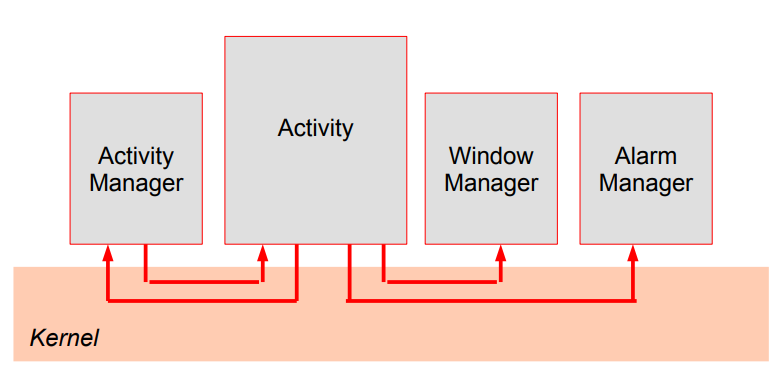
\includegraphics[width=400px,scale=0.5]{binder.PNG}
\\
Android Binder Es un mecanismo de comunicación interprocesos y un sistema de invocación remota de métodos que implementa a OpenBinder.
\\
Eso es un proceso de android puede llamar una rutina de otro proceso usando binder para identificar el método para invocar y pasar los argumentos entre procesos 
\\
Android no usa SysV IPC para comunicación entre procesos 
\\
La implementacion de binder está en: drivers/android/binder.c\newline
 con include file: include/uapi/linux/android/binder.h
\\
 
\includegraphics[width=400px,scale=0.5]{Capture.PNG}
 
 Como se puede ver en el diagrama de secuencia, primero debemos pedir un servicio al contexto, que en android es un contexto general para toda la aplicacion,a la vez que cada proceso también tiene su propio contexto, despues de eso podemos pedir servicios al API de Binder e interactuar los procesos de otro servicio en su contexto.

\subsection{Binder IPC. Binder userspace IPC; interfaces and AIDL}
\begin{itemize}
\item Author : Blancas Alva Efrain Jedahir
\end{itemize}	

\subsection{Aplicaciones en Android}
\begin{itemize}
\item Author : Candela Castellanos Pablo Antonio

\end{itemize}

\subsection{Aplicaciones en Android. Actividades}
\begin{itemize}
\item Author : Casas Monreal Juan, Rivera Sotomayor Luis Rafael
\end{itemize}

\subsection{Aplicaciones en Android. Servicios}
\begin{itemize}
\item Author : Cervantes Gónzalez Kevin, Rubio Lezama Eduardo
\end{itemize}

\subsection{Aplicaciones en Android. Receptores}
\begin{itemize}
\item Author : Chávez Muñoa Ian Eduardo
\end{itemize}

\subsection{Aplicaciones en Android. Proveedores de
contenidos}
\begin{itemize}
\item Author : Durán Pérez Gerardo Ezequiel
\end{itemize}

\subsection{Intents}
\begin{itemize}
\item Author : Espinosa Arista Abraham, Xie Yuguo
\end{itemize}

\subsection{Aplicacioness: Sandboxing}
\begin{itemize}
\item Author : Fuentes Juárez Francisco Javier Tonatiuh

\end{itemize}

\subsection{Seguridad}
\begin{itemize}
\item Author : Gaitan Dieguez Sandra Martha
\end{itemize}

\subsection{Seguridad}
\begin{itemize}
\item Author : García García Raúl Eduardo
\end{itemize}

\subsection{Modelo del proceso. Proceso inicial}
\begin{itemize}
\item Author : García García Ricardo
\end{itemize}



\newpage 
\textbf{\Large{2.2 \; Extensiones. wake locks}}\\[0.4em]

La administración de energía en dispositivos móviles es diferente que en la informática tradicional
De sistemas, por lo que Android agrega una nueva característica a Linux llamada wake locks para administrar cómo se va a dormir el sistema.\\
Los wakelocks son mecanismos de administración de energía que aseguran que su dispositivo Android no entre en modo de suspensión (que es el estado en el que debe esforzarse), porque una aplicación determinada necesita usar los recursos de su sistema i.e  las apps  se quedan abiertas en segundo plano y que fuerzan al dispositivo a funcionar incluso cuando tenemos la pantalla bloqueada o no estamos usando el dispositivo. \\
Dentro de los wakelocks podemos encontrarnos con dos tipos:\\

parciales \\                                                                                        son los que mantienen la CPU activa para que la aplicación en sí siga recopilando datos o funcionando incluso con el dispositivo bloqueado.                                                 Por ejemplo Gmail que notifica cuando llega un correo nuevo\\ 

Totales\\
son los que además de mantener la CPU activa, tienen despierta la pantalla.                                                                                                                         Ejemplo youtube que nos mantiene activa la pantalla sin tener que tocarla.\\

En un sistema informático tradicional, el sistema puede estar en uno de los dos posibles estados: ejecutándose y listo para la entrada del usuario, o profundamente dormido e incapaz de continuar ejecutando sin una interrupción externa como presionar una tecla de encendido\\
(falta mas info alrato la pongo XD)
Mientras corren piezas secundarias de hardware pueden encenderse o apagarse según sea necesario, pero el La CPU misma y las partes centrales del hardware deben permanecer en estado de alimentación para manejar tráfico de red entrante y otros eventos similares.\\

 Entrando en el sueño de menor poder el estado es algo que ocurre con relativa poca frecuencia: ya sea a través del usuario explícitamente
poner el sistema a dormir, o se va a dormir por sí mismo debido a un intervalo relativamente largo
de la inactividad del usuario. Salir de este estado de suspensión requiere una interrupción de hardware
desde una fuente externa, como presionar un botón en un teclado, en cuyo punto
el dispositivo se despertará y encenderá su pantalla
 en los dispositivos móviles  Aunque el usuario puede apagar la pantalla de una manera que parece poner el dispositivo a dormir.\\ Mientras la pantalla de un dispositivo está apagada, el dispositivo aún necesita
poder hacer trabajo: necesita poder recibir llamadas telefónicas, recibir y procesar
datos para los mensajes de chat entrantes, y muchas otras cosas.\\

Las expectativas sobre encender y apagar la pantalla de un dispositivo móvil también son
mucho más exigente que en una computadora tradicional. La interacción móvil tiende a
estar en muchas ráfagas cortas durante todo el día: recibe un mensaje y enciende el
dispositivo para verlo.\\
Teniendo en cuenta estos requisitos, una solución sería simplemente no llevar  la CPU a dormir cuando la pantalla de un dispositivo está apagada, de modo que siempre esté lista para retroceder de nuevo.  El núcleo, después de todo, sabe cuándo no hay ningún trabajo programado para hilos, y Linux (así como la mayoría de los sistemas operativos) hará automáticamente la CPU inactiva y usa menos energía en esta situación.
una CPU inactiva no es lo mismo que un verdadero sueño. Por ejemplo:

1-	En muchos chipsets (circuito integrado auxilial )  el estado inactivo usa mucha más potencia que un verdadero estado de sueño.

2-	Una CPU inactiva puede despertarse en cualquier momento si le sucede algo de trabajo estar disponible, incluso si ese trabajo no es importante.

3-	El simple hecho de que la CPU esté inactiva no le indica que puede apagar otro
hardware que no sería necesario en un verdadero sueño.\\

Los Wake locks en Android permiten que el sistema entre en un modo de espera más profundo, sin
estar vinculado a una acción explícita del usuario como apagar la pantalla. El estado por defecto
  del sistema con wake locks es que el dispositivo está dormido. 
Cuando el dispositivo esta  corriendo, para evitar que vuelva a dormirse, algo necesita estar teniendo un wake lock.
Mientras la pantalla está encendida, el sistema siempre mantiene un bloqueo de activación que evita que el dispositivo se vaya a dormir, por lo que seguirá funcionando, como esperamos.
Sin embargo, cuando la pantalla está apagada, el sistema en sí no tiene un wake lock
por lo que permanecerá fuera de sueño solo mientras algo más esté reteniendo.
Cuando no se mantienen más wake lock., el sistema se pone a dormir, y puede venir
fuera del sueño solo debido a una interrupción de hardware.\\



En un sistema operativo tradicional. Algunas fuentes de dicha interrupción son basadas en el tiempo de alarmas, eventos de la radio celular (como para una llamada entrante), entrante
tráfico de red, y presiona ciertos botones de hardware (como el botón de apagado).\\

 Los controladores de interrupción para estos eventos requieren un cambio de estándar                     Linux: necesitan adquirir un wake lock inicial para mantener el sistema en funcionamiento después de maneja la interrupción.\\
 
El  wake lock adquirido por un controlador de interrupción debe mantenerse el tiempo suficiente para transferir el control de la pila al controlador en el kernel que continuará procesando                           el evento. Ese controlador de núcleo es entonces responsable de adquirir su propio bloqueo de activación, después de lo cual, el bloqueo de activación de interrupción puede liberarse de manera segura sin riesgo de que el sistema volviendo a dormir


\newpage 

\textbf{\Large{2.3 \; Extensiones. Out-of-memory killer}}\\[0.4em]

Al utilizar un sistema existen situaciones donde la memoria puede llegar a ser extremadamente baja, para intentar recuperar el sistema de estos casos Linux provee de un \textit{out-of-memory killer}.\\

Situaciones de este tipo en sistemas operativos modernos son muy raras, ya que contamos con paginación y de \textit{swap}, así que es inusual que las aplicaciones se encuentren con fallas de \textit{out-of-memory}.\\

Esto no hace imposible que el kernel se encuentre en la situación donde no sea capaz de encontrar páginas de RAM disponibles cuando sean necesarias, no solo cuando queremos alocar memoria, también cuando se está haciendo de \textit{swap} o cuando se pagina en algún rango de direcciones que está siendo utilizado en el momento.\\

Para combatir estos casos de memoria baja el out-of-memory estándar de Linux es el último recurso para tratar de encontrar RAM y que el kernel continúe con la tarea que esté realizando.\\

Esto se logra asignando a los procesos un nivel de “badness” (maldad), y matar simplemente el proceso que es considerado el de mayor maldad.\\

La maldad de un proceso está basada en:

\begin{enumerate}
    \item Cantidad de RAM usada por el proceso
    \item Cuánto tiempo ha estado corriendo
    \item etc.
\end{enumerate}
El objetivo es matar procesos grandes que se espera no sean críticos.\\

Android necesita más del out-of-memory killer ya que no cuenta con un espacio de \textit{swap}, lo que lo hace más propenso a que se presenten una de estas situaciones, así que no hay otra forma de liberar memoria más que eliminando las páginas RAM limpias mapeadas desde el almacenamiento que han sido utilizadas recientemente.\\

Aún así, Android usa la configuración estándar del kernel de Linux para over-commit la memoria, esto es, permite que el espacio de direcciones se asigne en la RAM sin garantía de que haya RAM disponible para respaldarlo, ésta es una herramienta muy importante para optimizar el uso de memoria, ya que es común mapear archivos grandes donde solo tendrá que cargar en la RAM partes pequeñas del archivo.\\

Dada esta situación, el out-of-memory del Linux de serie no funciona bien para Android, pues está pensado más como un último recurso y tiene dificultades para correctamente identificar buenos procesos para eliminar.\\

Para combatir esto, Android crea su propio out-of-memory killer al kernel, con diferentes objetivos, este corre de forma mucho más agresiva, esto quiere decir que, cuando empieza a haber poca RAM.\\

Lo que se considera como poca RAM es un parámetro ajustable que indique cuánta memoria disponible y RAM cacheada en el kernel es aceptable. Cuando el sistema rebasa ese límite establecido entonces se ejecuta el \textit{out-of-memory killer} para liberar RAM, el objetivo de esto es asegurar que el sistema nunca se quede en malos estados de paginación, lo cual puede impactar negativamente la experiencia de usuario cuando aplicaciones en primer plano están compitiendo por RAM, ya que su ejecución se vuelve mucha más lenta debido a la continua paginación.\\

En vez de intentar adivinar cuál proceso debería ser matado, el \textit{out-of-memory killer} de Android se basa estrictamente en la información proporcionada por el espacio del usuario. \\
  
El out-of-killer tradicional tiene un parámetro \textit{oom\_adj} por cada proceso que puede ser usado para guiar hacía cuál es el mejor proceso puede ser matado modificando el score de maldad del proceso. \\ 
En cambio, la implementación de Android usa este mismo parámetro, pero como un ordenamiento estricto, procesos con el \textit{oom\_adj} más alto siempre serán matados antes que los que tienen uno más bajo. \\

El administrador de tareas es el indicado para asignar a cada proceso su \textit{oom\_adj}. \\v

\begin{center}
    \begin{tabular}{ | l | p{5cm} | l |}
    \hline
    \textbf{Categoria} & \textbf{Descripción} & \textbf{oom\_adj} \\ \hline
    SYSTEM & El sistema y proceso deamon  & -16 \\ \hline
    PERSISTENT & Procesos de aplicaciones siempre corriendo & -12 \\ \hline
    FOREGROUND & Actualmente interactuando con el usuario & 0 \\ \hline
    VISIBLE & Visible al usuario & 1 \\ \hline
    PERCEPTIBLE & Algo que el usuario sabe que está & 2 \\ \hline
    SERVICE & Servicios corriendo en el fondo & 3 \\ \hline
    HOME & El launcher  & 4 \\ \hline
    CACHED & Procesos que no están en uso & 5 \\ \hline
    \end{tabular}
\end{center}

Esto nos da el orden en que se matarán los procesos en un \textit{out-of-memory}, matará primero los procesos en caché, seguidos en el orden hacia arriba.

Adicionalmente emtenos los casos  en que el OOM evitará ser llamado  en un sistema Linux.\\
\begin{enumerate}
\item ¿Han pasado mas de 5 segundos desde la última falla? si sí, no se llama.
\item ¿Hay espacio suficiente para swap? si sí, no se llama.
\item Si no ha habido 10 fallas en los últimos 5 segundos. entonces no se llama.
\item ¿Se ha fallado en el último segundo? si no, no se llama.
\item
Un proceso ha sido matado en los últimos 5 segundos? si sí, no se llama.
\\
\end{enumerate}
Entiéndase fallo como no haber podido liberar memoria sin usar OOM.
\newpage
\textbf{\Large{2.12 \; Aplicaciones en Android}}\\[0.4em]
\begin{itemize}
\item \textbf{¿Que es una aplicacion?} \\ \\
En Android las aplicaciones no son archivos ejecutables con un punto de entrada principal si no que es un contenedor de todo lo que compone esa aplicación (como lo son el código, recursos, gráficos y otros datos para el sistema). Por convención estas aplicaciones tienen la extensión apk (Android application package por sus sglas en ingles), el cual es un archivo zip normal que contiene todo sobre la aplicación. \\ 
\end{itemize}

Los contenidos importantes de un apk son:
\begin{enumerate}

\item	Un archivo manifiesto(AndroidManifest.xml) que describe que es la aplicación, que hace y como ejecutarla. Este archivo debe proporcionar un nombre de paquete para la aplicación y una cadena de estilo de java que lo identifica de forma única.

\item Los recursos necesarios para la aplicación, en donde se incluyen mapas de bits, descripciones etc.

\item El código fuente de la aplicacion en si.

\item Identificación de la firma, que es una identificación segura del autor de la aplicación. 

\end{enumerate}


\begin{itemize}
\item \textbf{¿Y entonces como inician las aplicaciones?} \\ \\
Como la aplicación Android no tienen un punto de entrada principal, en su lugar inician bajo la etiqueta <aplication> en el archivo AndroidManifest.xml y una variedad de puntos de entrada que describen la cosas que la aplicación puede hacer. Esos tipos de entrada son: Actividad, receptor, servicio y proveedor de contenido. Cada uno de estos tipos de componentes diferentes que puede contener una aplicación tiene diferentes semánticas y usos dentro del sistema. 
\end{itemize}


\begin{itemize}
\item \textbf{Administrador de paquetes} \\ \\
El administrador de paquetes es la parte de Android que realiza un seguimiento de todos los paquetes de aplicaciones. Analiza el manifiesto de todas las aplicaciones, recopilando e indexando la información que encuentra en ellas. Con esa información, proporciona facilidades para que los clientes la consulten sobre las aplicaciones instaladas actualmente y recuperen información relevante sobre ellas. También es responsable de instalar aplicaciones (crear espacio de almacenamiento para la aplicación y garantizar la integridad de la aplicación) así como todo lo necesario para desinstalar (limpiar todo lo relacionado con una aplicación previamente instalada).
Las aplicaciones declaran de forma estática sus puntos de entrada en su manifiesto para que no necesiten ejecutar código en el momento de la instalación, este diseño hace que el sistema sea más robusto ya que la instalación de una aplicación no requiere la ejecución de ningún código de aplicación, las capacidades de nivel superior de la aplicación siempre se pueden determinar mirando el manifiesto, no hay necesidad de mantener una base de datos separada de esta información  y garantiza que no quede información sobre una aplicación después de que se desinstala. Esto es de gran ayuda para cumplir con el diseño de compatibilidad de interoperación y colaboración entre aplicaciones. Las aplicaciones pueden publicar piezas de sí mismas que proporcionan funcionalidades específicas, que otras aplicaciones pueden usar directa o indirectamente.
Sobre el gestor de paquetes se encuentra otro importante servicio del sistema, el administrador de actividades es el que se encarga de determina cuándo, dónde y cómo deben ejecutarse las aplicaciones, en realidad es el responsable de ejecutar los cuatro tipos de componentes de la aplicación e implementar el comportamiento apropiado para cada uno de ellos.
\end{itemize}



\newpage
\textbf{\Large{2.12 \; Intent}}\\[0.4em]
\begin{itemize}
\item \textbf{Que es intent} \\ \\
Intent es un objeto muy importante de android, para iniciar los 
componentes y transferir \\[0.3em] los datos entre los componentes, se existe en mayorias los programas. \\ 
\end{itemize}

\begin{itemize}
\item \textbf{Los contenidos del intent} \\ \\
El intent es un objeto de información, la parte crucial de el son las informaciones que  \\[0.3em] contiene, de hecho no importa de ser implicta o explicita, cuando se manda un intent, el \\[0.3em] comportamiento del sistema corresponde la combinación de las informaciones del intent, \\[0.3em] las informaciones de un intent como el siguiente imagen:
\end{itemize}

 


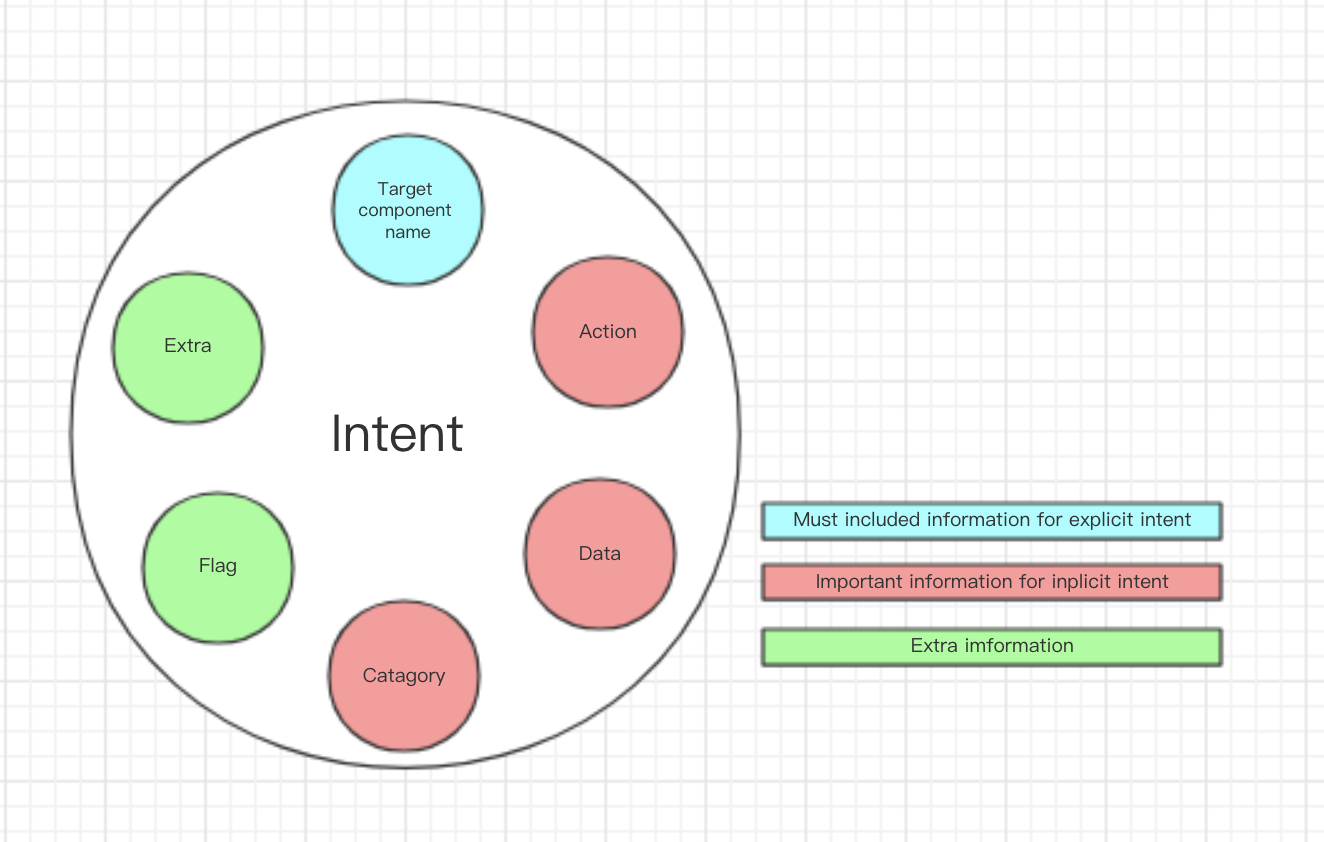
\includegraphics[width=5in]{intent.png}


\begin{itemize}
\item \textbf{Nombre del componente de destino} \\ \\
El nombre es la information necesaria para intent explicito, se mandará al componente \\[0.3em] especifíca(por eso es explícito), si no, el systema filtra todos los componentes que pueden \\[0.3em] responder el intent(implicito). Se puede usar setComponent(), setClass(), setClassName() , \\[0.3em] etc para asignar el nombre del componente. \\ 

\item \textbf{Contenido de intent - Action} \\ \\
Eso significa las acciones principales que manda de un intent a los componentes, por \\[0.3em] ejemplo: la acción principal de una aplicación de imagen es 
checar la imagen, y ver la \\[0.3em] localidad para una aplicación de map.. En general se usa las acciones defaultas de android \\[0.3em] más, aqui introducimos algunas aciones defaultas :

\begin{itemize}
  \item{ACTION\_VIEW}  \\[0.6em] 
Para mostrar alguna vista al usuario, por ejemplo, abre un sitio de web con navegador, \\[0.3em] o  abre una imagen con una aplicación de foto, etc.
   \item{ACTION\_SEND} \\[0.6em]
Para mandar los datos, por ejemplo el correo electronico ó alguna aplicación de red \\[0.3em] social.

   \item{ACTION\_DIAL} \\[0.6em]
Para mostrar una pantalla con teclado telefonico, para que el usuario puede hacer la \\[0.3em] llamada.\\ \\ \\
\textbf{Más acciones defaultas se encuetra en este sitio : \\[0.7em] }
https://developer.android.com/reference/android/content/Intent \\
\end{itemize}

\end{itemize}

\begin{itemize}
\item \textbf{Contenido de intent - Data} \\[-0.2em]

Incluye objeto de uri y memitype dos partes, el contenido de Data depende acción en general,\\[0.3em] por ejemplo si acción es ACTION\_VIEW, entonces Data  podriá ser la liga de un sitio web, \\[0.3em]tambien puede ser uri con tipo de dato de la imagen.
Cuando asigna Uri y MIME en mismo \\[0.3em] tiempo ayudariá Android a buscar el mejor componente para responder el intent, por ejemplo \\[0.3em] hay muchos componentes pueden responder ACTION\_VIEW, navegador, player, aplicación \\[0.3em] de imagen etc. En este caso si configura mimeType como "image/jpeg" ó "video/mp4", el \\[0.3em] sistema podrá eligir el mejor componente para responder. \\

\end{itemize}


\begin{itemize}
\item \textbf{Catagory} \\ \\
Es la cadena del tipo del componente destino, un intent puede agregar varios Catagory, aqui listamos las catagory mas comunes :

\begin{itemize}
  \item{CATEGORY\_BROWSABLE}  \\[0.6em] 
La \textit{Activity} permite iniciar a su mismo a través el navegador, para mostrar los datos de  \\[0.3em]  la liga, por ejemplo imagen o correo electronico. \\ 
   \item{CATEGORY\_LAUNCHER}  \\[0.6em]
Esta \textit{Activity} es la \textit{Activity} inicial de la tarea, esta en la lista del iniciador de sistema.  \\[0.6em]

\textbf {Esas 4 que estan arriba (Nombre del componente de destino, Action, Data, \\[0.3em] Category) pueden afectar el resuelto de intent para determinnar cual \\[0.3em] componente se usa el sistema en final, ahora introducimos otro dos más, que \\[0.3em] no afecta el sistem inicia componente(Extra y Flag).} \\
\end{itemize}

\end{itemize}

\begin{itemize}
\item \textbf{Extra} \\ \\
El intent lleva los datos extras tmabien es una manera común para transferir la \\[0.3em] información, se usa los metodos de putExtra() para agregar dato extra, y cada metodo recibe \\[0.3em] dos parametros, llave y valor. Tambien se puede crear un objeto de Bundle, despues usa \\[0.3em] putExtras() para insertar Bundle al intent. \\

\item \textbf{Flag} \\ \\
Lo que hace Flag es indicar el sistema como iniciar \textit{Activity}, por ejemplo, \textit{Activity} debe \\[0.3em] pertenecer en cual tarea, y que va a hacer despues iniciarla.\\

\item \textbf{Metodos de constructores} \\ \\
Aqui son unos ejemplos de obtener el objeto de intent. \\[0.7em]
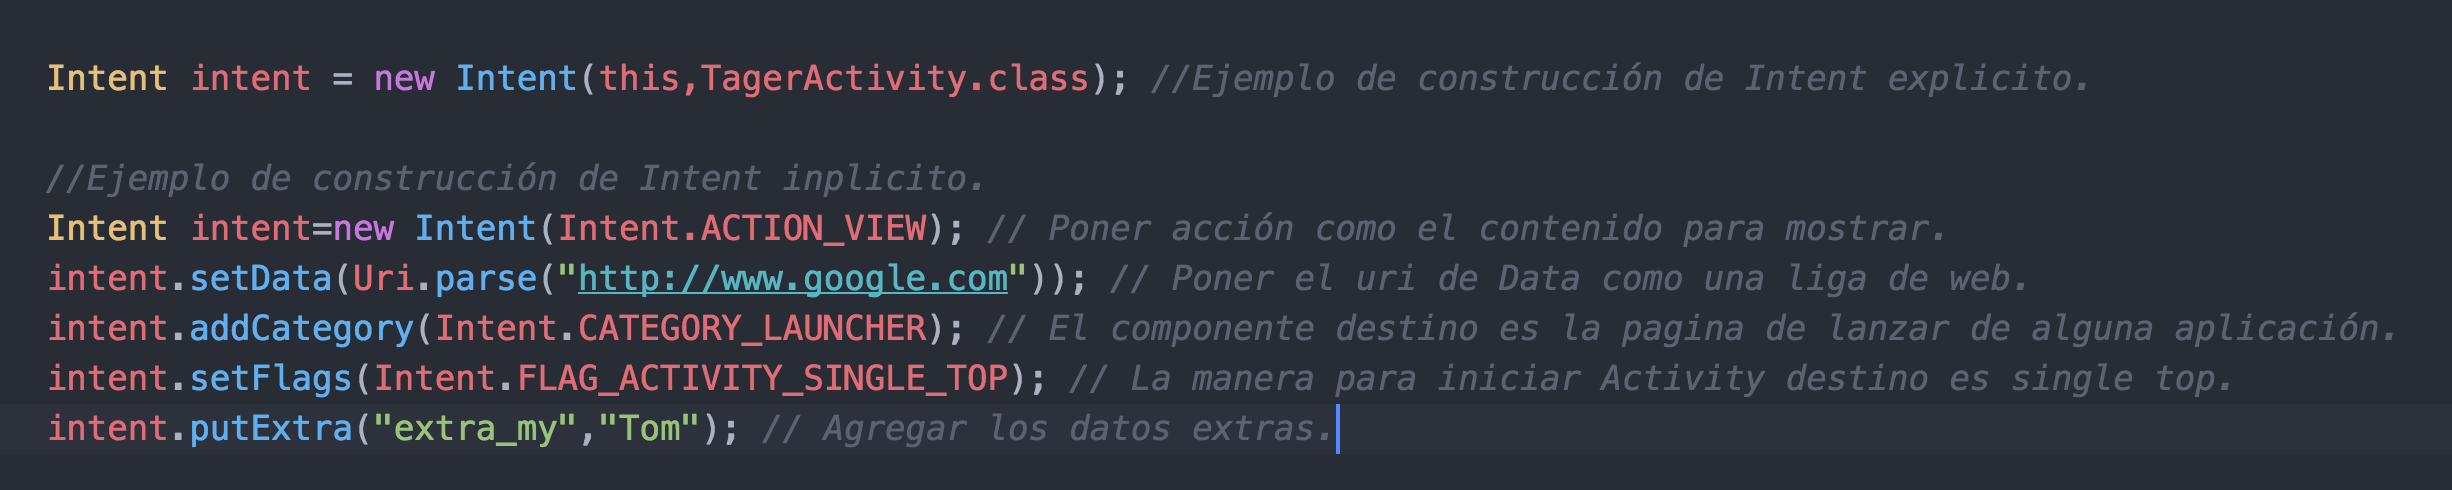
\includegraphics[width=6in]{Metodo_de_constructor.png}
\end{itemize}



\textbf{\Large{2.13 \; Aplicaciones: Sandboxing}}\\[0.4em]
 
 La plataforma Android se aprovecha de la protección basada en el usuario Linux como un medio para identificar y aislar los recursos de aplicaciones. Este sistema operativo asigna un identificador único de usuario (UID) de cada aplicación Android y lo ejecuta como ese usuario en un proceso separado. Este enfoque es diferente de otros sistemas operativos, incluyendo la configuración de Linux tradicionales, donde múltiples aplicaciones se ejecutan con los mismos permisos de usuario. Esto establece un nivel de kernel Aplicación Sandbox. El kernel aplica la seguridad entre las aplicaciones y el sistema en el nivel de proceso a través de las instalaciones de Linux estándar, como los ID de usuario y de grupo que se asignan a las aplicaciones. Por defecto, las aplicaciones no pueden interactuar entre sí y las aplicaciones tienen un acceso limitado al sistema operativo. \\
 
Si la aplicación “A” intenta hacer algo malicioso como leer datos de la aplicación de “B” o marque el teléfono sin permiso, que es una aplicación independiente, entonces el sistema operativo protege contra esto porque la aplicación “A” no tiene los privilegios de usuario apropiados.\\


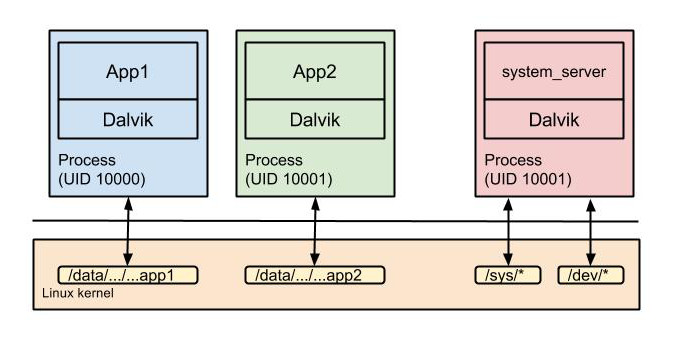
\includegraphics[width=400px,scale=0.5]{app.jpg}


El sandbox es simple, auditable, y en base a décadas de experiencia, la separación de usuario de estilo UNIX de los procesos y los permisos de archivos. Desde que la aplicación Sandbox está en el núcleo del programa, este modelo de seguridad se extiende a código nativo y para aplicaciones de sistemas operativos. Todo el software por encima del kernel, incluidas las bibliotecas del sistema operativo, marco de aplicación, tiempo de ejecución de aplicaciones y todas las demás aplicaciones, se ejecutan dentro de la aplicación Sandbox. En algunas plataformas, los desarrolladores se ven obligados a un marco de desarrollo específico, un conjunto de APIs o el lenguaje, con el fin de reforzar la seguridad. En Android no hay restricciones sobre cómo una aplicación puede ser escrita y que son necesarias para reforzar la seguridad. A este respecto, el código nativo es tan seguro como el código interpretado\\



En algunos sistemas operativos, los errores de corrupción de memoria conducen generalmente a comprometer por completo la seguridad del dispositivo. Este no es el caso en Android debido a todas las aplicaciones y sus recursos están dentro del objeto de seguridad en el nivel de sistema operativo. Un error de corrupción de memoria sólo permitirá la ejecución de código arbitrario en el contexto de esa aplicación en particular, con los permisos establecidos por el sistema operativo. Al igual que todos los elementos de seguridad, la aplicación Sandbox no es irrompible e invulnerable a posibles ataques. Sin embargo, para salir de la aplicación Sandbox en un dispositivo configurado correctamente, se debe poner en peligro la seguridad del kernel de Linux.\\

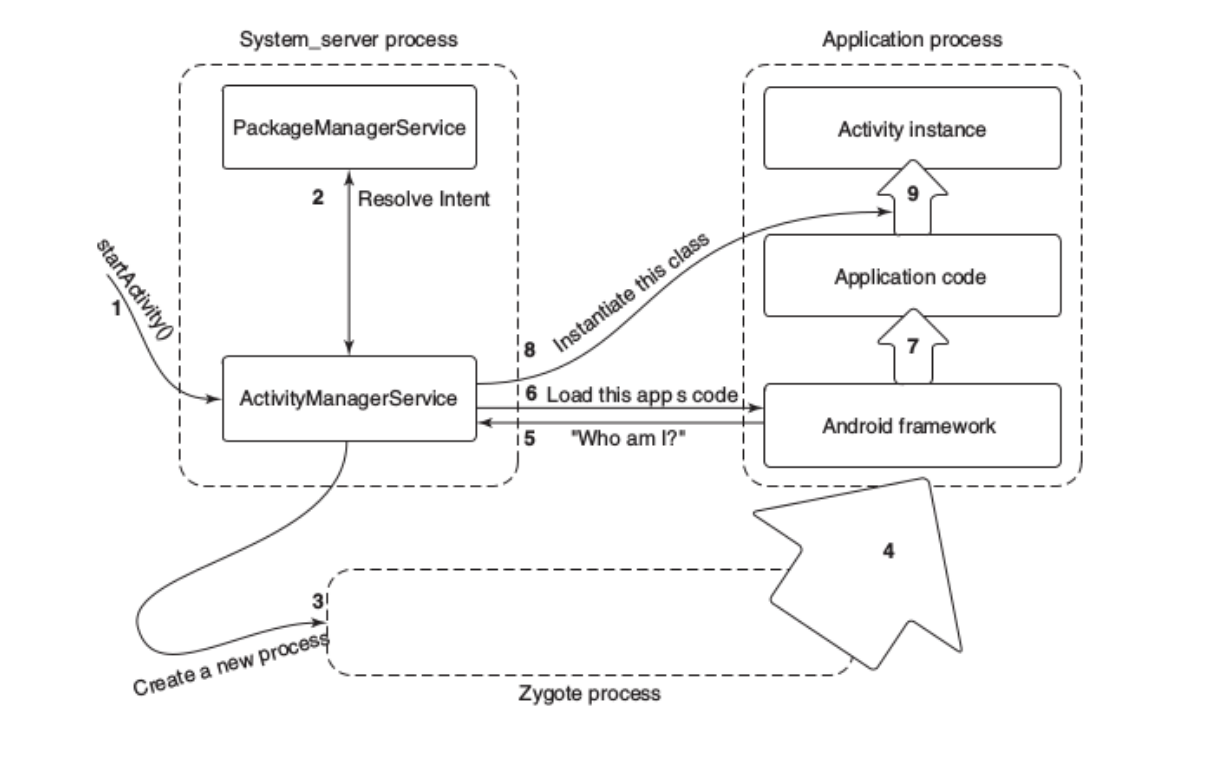
\includegraphics[width=200px,scale=0.5]{sandbo.png}
\\


\textbf{\Large{2.15 \; Seguridad}}\\[0.4em]

Tradicionalmente en los sistemas operativos, las aplicaciones se ven como la ejecución de código como el usuario, en nombre del usuario. Este comportamiento ha sido heredado de la linea de comandos, donde ejecuta el comando ls y espera que se ejecute como su identidad (UID), con los mismos derechos de acceso que tiene en el sistema. De la misma manera, cuando utiliza una interfaz gráfica de usuario para iniciar un juego que quieras jugar, ese juego será efectivo ejecutar como su identidad, con acceso a sus archivos y muchas otras cosas que puede que en realidad no lo necesite.
Sin embargo, esto no es la forma en que usamos las computadoras en la actualidad. Ejecutamos aplicaciones que adquirimos de una fuente de terceros menos confiable, que han barrido funcionalidad, que hará una gran variedad de cosas en su entorno sobre el que tienen poco control. Hay una desconexión entre el modelo de la aplicación compatible
por el sistema operativo y el que realmente está en uso. Esto puede ser mitigado
mediante estrategias tales como distinguir entre los privilegios de usuario normales y '' admin ''y advirtiendo la primera vez que ejecutan una aplicación.\\
En otras palabras, los sistemas operativos tradicionales son muy buenos para proteger a los usuarios de otros usuarios, pero no para proteger a los usuarios de ellos mismos. Todos los programas se ejecutan con el poder del usuario y, si alguno de ellos se porta mal, puede hacer todo bastante daño. Puede filtrar toda la información accesible para el usuario. Tú podrías ejecutar rm -rf * para obtener un buen directorio de inicio vacío. Y si el programa
no solo es un error, sino también malicioso, podría encriptar todos tus archivos para pedir un rescate.
¡Ejecutar todo  es peligroso!\\

La seguridad de las aplicaciones en Android gira en torno a los UID. En Linux, cada proceso
se ejecuta como un UID específico, y Android usa el UID para identificar y proteger la seguridad conbarreras. La única forma de interactuar entre procesos es mediante algún mecanismo de IPC, que generalmente lleva consigo suficiente información para identificar el UID del llamador. Binder IPC incluye explícitamente esta información en cada transacción entregada en todos los procesos para que un destinatario del IPC pueda solicitar fácilmente el UID
.
Android predefine varios UID estándar para las partes de nivel inferior de
sistema, pero a la mayoría de las aplicaciones se les asigna dinámicamente un UID, al primer arranque o en tiempo de instalación, desde un rango de '' UIDs de aplicación ''.

\begin{center}
    \begin{tabular}{ | l | p{5cm}|}
    \hline
    \textbf{UID} & \textbf{Proposito}  \\ \hline
    0 & Root   \\ \hline
    1000 & Nucleo del sistema \\ \hline
    1001 & Servicios de telefonia \\ \hline
    1013 & Procesos de medios de bajo nivel \\ \hline
    2000 &  Acceso a la linea de comandos\\ \hline
    10000-19999 &  Aplicaciones UID dinamicamente asignadas\\ \hline
    100000 & Inicio de usuarios secundarios  \\ \hline
    \end{tabular}
\end{center}

Cuando a una aplicación se le asigna por primera vez un UID, se crea un nuevo directorio de almacenamiento para ello, con los archivos que posee su UID. La aplicación obtiene acceso libre a sus archivos privados allí, pero no puede acceder a los archivos de otras aplicaciones.\\
Incluso el propio sistema, que se ejecuta como UID 1000, no puede tocar los archivos de las aplicaciones. Esta es la razón por la que existe el daemon installd: se ejecuta con privilegios especiales para ser capaz de acceder y crear archivos y directorios para otras aplicaciones. Hay un API installd muy restringida proporciona al administrador de paquetes para que cree y administre los directorios de datos de las aplicaciones según sea necesario.
En su estado base, los entornos limitados de aplicación de Android deben rechazar cualquier tipo de interacciones entre aplicaciones que puedan violar la seguridad entre ellas. Esto podría ser para la robustez (evitando que una aplicación bloquee otra aplicación), pero la mayoría de las veces es sobre el acceso a la información.\\

Los permisos no están vinculados a proveedores de contenido; cualquier IPC en el sistema puede ser protegido por un permiso a través del sistema preguntando al administrador del paquete si el quien llama tiene el permiso requerido.\\

El sandbox se basa en procesos y UID, por lo que una barrera de seguridad siempre ocurre en un límite del proceso, y los permisos están asociados con UID. Dado esto, un permiso
y la verificación se pueden realizar recuperando el UID asociado con el IPC entrante
y preguntando al administrador del paquete si ese UID ha recibido el correspondiente
permiso. Por ejemplo, los permisos para acceder a la ubicación del usuario son
impuestos por el servicio de administrador de ubicación del sistema cuando las aplicaciones llaman a él.\\






\textbf{\Large{2.16 \; Modelo del Proceso: Proceso Inicial}}\\[0.4em]
 
Android tiene como base el núcleo de Linux. Sabemos que un modelo de proceso en Linux es\textbf{fork} el cual nos es util en la creación de un nuevo proceso y después \textbf{exec} para ejecutarlo. \textbf{Shell} por su parte gestiona estas acciones. Resulta ser que en el Sistema Operativo Android, este proceso tiene variaciones.\\
	
    {Para lanzar un nuevo proceso, el administrador de actividades debe comunicarse con \textbf{zygote}. \newline 
 	Cuándo el administrador de actividades comienza, se crea un socket con 				\textbf{zygote}. A través de este socket se mandan comandos cuando se necesita inicar un nuevo proceso. Este comando describe principalmente el \textbf{sandbox} que será creado: La \textbf{UID} que el nuevo proceso debe correr y alguna restricción de seguridad. Así \textbf{zygote} debe ejecutarse como \textbf{root}: Cuando \textbf{zygote} realiza un \textbf{fork}, hace las configuraciones apropiadas para que el UID corra también como root, finalmente deja los privilegios de root y cambia el proceso a la UID deseada.\\ \newline Como se ha visto en secciones anteriores acerca de las aplicaciones de Android, el administrador de actividades mantiene información dinámicamente acerca de la ejecución de actividades, servicios, emisiones y proveedores de contenido. Utiliza esta información para manejar la creación y gestión de procesos de aplicación. Por ejemplo, cuando el lanzador de aplicaciones llama al sistema con un nuevo intento de iniciar una nueva actividad, es el manejador de actividades el responsable para que esta aplicación corra correctamente.\\

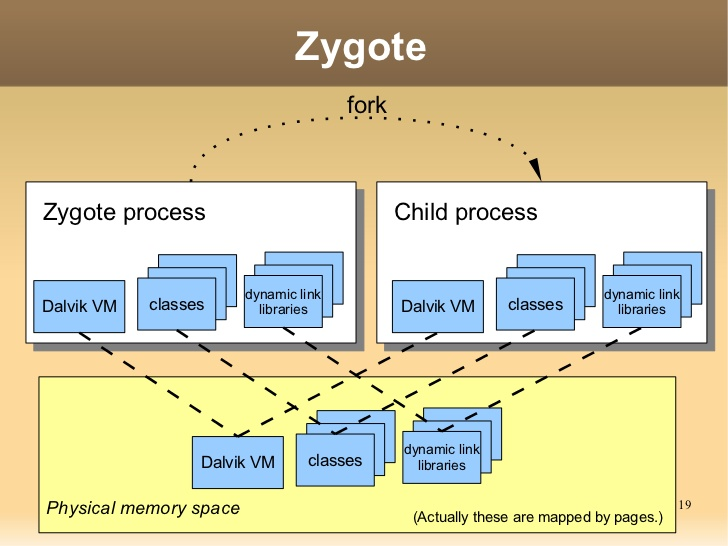
\includegraphics[width=400px,scale=0.3]{zyg.jpg}\\
 

El flujo para que un proceso comience su ejecución es el siguiente: \\
\begin{itemize}
  \item Proceso actual que realiza una llamada al administrador de actividades describiendo la tarea nueva a ejecutar.
  \item Administrador de actividades solicita al administrador del paquete la resolución en paquetes explícitos.
  \item El manejador de actividades determina que no está en ejecución esa actividad y le pide a \textbf{zygote} un nuevo proceso del UID apropiado.
  \item \textbf{Zygote} realiza un \textbf{fork}, genera un proceso nuevo (replica de sí mismo), restringe privilegios y le asigna una UID adecuada para el \textbf{sandbox} de la aplicación y concluir la inicialización de \textbf{Dalvik} en ese proceso, así Java se está ejecutando por completo, con el ambiente de Java y ejecutándose, pregunta por la tarea a realizar al manejador de actividades.
  \item El manejador de actividades envía toda la información disponible.
  \item El proceso carga el código de la aplicación en ejecución.\\
  \item El mandejador de aplicaciones envía al nuevo proceso alguna operación pendiente.
  \item El proceso nuevo recibe la información, crea instancias de las clases apropiadas de Java y las ejecuta.\\
\end{itemize}}




\begin{center}

\end{center}
  

\end{document}